\subsection{\texorpdfstring{Characterization of measures with base \(\mu\)}{Characterization of measures with base mu}}

THEOREM 2 (Lebesgue--Nikodym). --- Let \(\mu\) and \(\nu\) be two positive measures on T. The following properties are equivalent:

\begin{enumerate}
\def\labelenumi{\arabic{enumi})}
\item
  \(\nu\) is a measure with base \(\mu\) .
\item
  Every locally \(\mu\) -negligible set is locally \(\nu\) -negligible.
\item
  Every \(\mu\) -negligible compact set is \(\nu\) -negligible.
\end{enumerate}

It is clear that 1) implies 2) (Cor. 1 of Prop. 3), and that 2) implies 3). We are going to show that 3) implies 1). We first note that if the condition 3) is satisfied, then every set A that is universally measurable and locally \(\mu\) -negligible is locally \(\nu\) -negligible; for, \(\nu^{\bullet}(\mathrm{A}) = \sup \nu(\mathrm{K})\) , where K runs over the set of compact sets contained in A ( \(\S 1\) , No.~3, Prop. 10, a) and Ch. IV, \(\S 4\) , No.~6, Cor. 2 of Th. 4). Next, we shall establish two lemmas.

Lemma 2. --- Let \(\alpha\) be a bounded positive measure on T, and \(\beta\) a real measure on T such that \(|\beta| \leqslant M\alpha\) , where M is a positive constant. Then, there exists a real function \(u\) , \(\alpha\) -integrable, such that \(\beta = u \cdot \alpha\) .

Let \(g\) be an element of the space \(\mathcal{L}_{\mathbf{R}}^{2}(\mathrm{T},\alpha)\) ; \(g\) is \(\beta\) -measurable and \(\int^{\bullet}|g|^2 d|\beta| \leqslant \mathrm{M}\int^{\bullet}|g|^2 d\alpha < +\infty\) . The function \(g\) therefore belongs to \(\mathcal{L}^2 (\mathrm{T},|\beta|)\) , and also to \(\mathcal{L}^1 (\mathrm{T},|\beta|)\) since \(\beta\) is bounded. By the Cauchy-Schwarz inequality,

\[
| \beta (g) | ^ {2} \leqslant \left(\int | g | d | \beta |\right) ^ {2} \leqslant \left(\int d | \beta |\right) \left(\int | g | ^ {2} d | \beta |\right) \leqslant \mathrm{M} ^ {2} \alpha (1) \alpha (| g | ^ {2}).
\]

The mapping \(g \mapsto \beta(g)\) is thus a continuous linear form on \(\mathcal{L}^2(\mathrm{T},\alpha)\) . The Hausdorff space associated with \(\mathcal{L}^2(\mathrm{T},\alpha)\) being a Hilbert space, there then exists (TVS, Ch. V, §1, No.~7, Th. 3) a real function \(u \in \mathcal{L}^2(\mathrm{T},\alpha)\) , therefore also belonging to \(\mathcal{L}^1(\mathrm{T},\alpha)\) , such that \(\beta(g) = \alpha(ug)\) for every \(g \in \mathcal{L}^2(\mathrm{T},\alpha)\) . Applying this relation for \(g \in \mathcal{K}(\mathrm{T})\) , one sees that \(\beta = u\cdot \alpha\) .

Lemma 3. --- Suppose that the positive measure \(\nu\) is such that every \(\mu\) -negligible compact set is \(\nu\) -negligible. Let \(\mathfrak{K}\) be the set of compact subsets \(K\) of \(T\) having the following property:

\begin{enumerate}
\def\labelenumi{(\arabic{enumi})}
\setcounter{enumi}{10}
\tightlist
\item
  There exists a constant \(M \geqslant 0\) such that \(\varphi_{K} \cdot \nu \leqslant M \varphi_{K} \cdot \mu\) . The set K is then \(\mu\) -dense in T.
\end{enumerate}

If K satisfies (11), and if A is a Borel set contained in K, it follows at once from Prop. 8 that \(\varphi_{\mathrm{A}} \cdot \nu \leqslant \mathrm{M}\varphi_{\mathrm{A}} \cdot \mu\) ; from this, one deduces that the union of two elements K, \(K'\) of \(\mathfrak{K}\) belongs to \(\mathfrak{K}\) because \(\varphi_{\mathrm{K} \cup \mathrm{K}'} = \varphi_{\mathrm{K}} + \varphi_{\mathrm{A}}\) , where \(\mathrm{A} = \mathrm{K}' \cap \mathbb{C}\mathrm{K}\) . To establish the lemma, it remains to prove that every compact set L such that \(\mu(\mathrm{L}) > 0\) contains a compact set \(\mathrm{K} \in \mathfrak{K}\) such that \(\mu(\mathrm{K}) > 0\) (Ch. IV, §5, No.~8, Prop. 12). Choose a number \(\mathrm{M} > \nu(\mathrm{L}) / \mu(\mathrm{L})\) and apply Lemma 1 to the bounded positive measure \(\alpha = \varphi_{\mathrm{L}} \cdot (\nu + \mathrm{M}\mu)\) and the measure \(\beta = \varphi_{\mathrm{L}} \cdot (\nu - \mathrm{M}\mu)\) . Replacing if necessary the function \(u\) such that \(\beta = u \cdot \alpha\) by a function equal to it \(\alpha\) -almost everywhere, one can suppose that \(u\) is universally measurable (§3, No.~4, Prop. 7) and is zero outside of L. The set H of \(t \in \mathrm{T}\) such that \(u(t) < 0\) , which is contained in L, could not be \(\mu\) -negligible, for it would then be \(\nu\) -negligible (by the remark made at the beginning of the proof of Th. 2), hence \(\alpha\) -negligible, and one would have \(\beta(\mathrm{L}) > 0\) , which contradicts the choice of M. Let K be a compact set contained in H, such that \(\mu(\mathrm{K}) > 0\) ; let us show that \(\mathrm{K} \in \mathfrak{K}\) , which will establish the lemma. By Prop. 8,

\[
\varphi_ {\mathrm{K}} \cdot (\nu - \mathrm{M} \mu) = \varphi_ {\mathrm{K}} \cdot \beta = \varphi_ {\mathrm{K}} \cdot (u \cdot \alpha) = (\varphi_ {\mathrm{K}} u) \cdot \alpha .
\]

The function \(\varphi_{\mathbf{K}}u\) is negative, therefore we indeed have \(\varphi_{\mathbf{K}}\cdot \nu \leqslant \mathrm{M}\varphi_{\mathbf{K}}\cdot \mu\) .

Let us now complete the proof of Theorem 2. Assume that the condition 3) is verified and define \(\mathfrak{K}\) as in Lemma 3. Let \((\mathrm{K}_{\alpha})_{\alpha \in \mathbf{A}}\) be a locally countable family of pairwise disjoint elements of \(\mathfrak{K}\) , such that the set \(\mathrm{N} = \mathrm{T} - \bigcup_{\alpha \in \mathbf{A}} \mathrm{K}_{\alpha}\) is locally \(\mu\) -negligible (Ch. IV, §5, No.~9, Prop. 14); the family \((\mathrm{K}_{\alpha})\) being locally countable, N is universally measurable and therefore locally \(\nu\) -negligible. Set \(\mu_{\alpha} = \varphi_{\mathrm{K}_{\alpha}} \cdot \mu\) , \(\nu_{\alpha} = \varphi_{\mathrm{K}_{\alpha}} \cdot \nu\) ; since the functions \(\varphi_{\mathrm{K}_{\alpha}}\) form a locally countable family, whose sum is equal to 1 locally almost everywhere for \(\mu\) and for \(\nu\) , Proposition 6 implies that \(\mu = \sum_{\alpha \in \mathbf{A}} \mu_{\alpha}\) , \(\nu = \sum_{\alpha \in \mathbf{A}} \nu_{\alpha}\) . On the other hand, by the definition of \(\mathfrak{K}\) , there exists for every \(\alpha\) a constant \(\mathrm{M}_{\alpha}\) such that \(\nu_{\alpha} \leqslant \mathrm{M}_{\alpha} \mu_{\alpha}\) ; Lemma 2 therefore implies the existence of a function \(g_{\alpha}\) , which one can suppose to be zero outside of \(\mathrm{K}_{\alpha}\) and positive (Cor. 3 of Prop. 3), such that \(\nu_{\alpha} = g_{\alpha} \cdot \mu_{\alpha}\) . Therefore (No.~4, Prop. 8)

\[
\nu_ {\alpha} = g _ {\alpha} \cdot \mu_ {\alpha} = g _ {\alpha} \cdot (\varphi_ {\mathrm{K} _ {\alpha}} \cdot \mu) = (g _ {\alpha} \varphi_ {\mathrm{K} _ {\alpha}}) \cdot \mu = g _ {\alpha} \cdot \mu .
\]

Set \(g = \sum_{\alpha \in A} g_{\alpha}\) ; since the family \((g_{\alpha})\) is locally countable and the family \((\nu_{\alpha})\) is summable, Proposition 6 implies that \(g\) is locally \(\mu\) -integrable, and that \(\nu = g \cdot \mu\) , which establishes the theorem.

COROLLARY 1. --- Let N be a set of positive measures with base \(\mu\) , admitting a supremum \(\nu\) in \(\mathcal{M}(\mathrm{T})\) ; then \(\nu\) is a measure with base \(\mu\) .

The Cor. of Prop. 2 permits reduction to the case that N is an increasing directed set. For every locally \(\mu\) -negligible set A one then has, by Prop. 11 of §1, No.~4,

\[
\nu^ {\bullet} (\mathrm{A}) = \sup _ {\lambda \in \mathcal {N}} \lambda^ {\bullet} (\mathrm{A}) = 0.
\]

Theorem 2 therefore implies that \(\nu\) is a measure with base \(\mu\) .

COROLLARY 2. --- Let \(\nu\) be a real measure on T. In order that \(\nu\) belong to the band generated by \(\mu\) in the fully lattice-ordered space \(\mathcal{M}(\mathrm{T})\) (Ch. II, §1, No.~5), it is necessary and sufficient that \(\nu\) be a measure with base \(\mu\) .

On considering \(\nu^{+}\) and \(\nu^{-}\) , one is immediately reduced to the case of a positive measure \(\nu\) (No.~2, Cor. of Prop. 2). Let us then set \(\nu_{n} = \inf(n\mu, \nu)\) ; \(\nu\) belongs to the band generated by \(\mu\) if and only if \(\nu = \sup_{n} \nu_{n}\) (Ch. II, §1,

No.~5, Cor. of Prop. 6). Now \(\nu_{n}\) , being bounded above by \(n\mu\) , is a measure with base \(\mu\) by Th. 2; the relation \(\nu = \sup_{n} \nu_{n}\) therefore implies that \(\nu\) is

a measure with base \(\mu\) (Cor. 1). Conversely, suppose that \(\nu\) is a measure with base \(\mu\) : \(\nu = g \cdot \mu\) , where \(g\) is locally \(\mu\) -integrable and positive. Then \(\nu_n = \inf(g, n) \cdot \mu\) (Cor. of Prop. 2), and it follows at once from Lebesgue's theorem (Ch. IV, §4, No.~3, Prop. 4) that \(\nu = \sup_{n} \nu_n\) .

COROLLARY 3. --- Let \(\theta\) be a complex measure; there exists a universally measurable function \(v\) , with \(|v| = 1\) , such that \(\theta = v \cdot |\theta|\) , \(|\theta| = \overline{v} \cdot \theta\) .

Write \(\theta = \theta_{1} - \theta_{2} + i(\theta_{3} - \theta_{4})\) , where \(\theta_{1} = (\mathcal{R}\theta)^{+}\) , \(\theta_{2} = (\mathcal{R}\theta)^{-}\) , \(\theta_{3} = (\mathcal{I}\theta)^{+}\) , \(\theta_{4} = (\mathcal{I}\theta)^{-}\) ; the positive measures \(\theta_{i} (i = 1, 2, 3, 4)\) , being bounded above by \(|\theta|\) (Ch. III, §1, No.~6, formula (17)), are measures with base \(|\theta|\) by Theorem 2. It follows that there exists a locally \(|\theta|\) -integrable function v such that \(\theta = v \cdot |\theta|\) . Proposition 2 then yields the relation \(|\theta| = |v| \cdot |\theta|\) , which implies that \(|v| = 1\) locally \(|\theta|\) -almost everywhere (Cor. 2 of Prop. 3). Finally, by Prop. 8, \(\overline{v} \cdot \theta = (v\overline{v}) \cdot |\theta| = |\theta|\) . Since the function v is defined only up to a locally \(|\theta|\) -negligible function, one can suppose that v is universally measurable (§3, No.~4, Prop. 7) and that \(|v| = 1\) everywhere.

Remarks. --- 1) Suppose that \(\lambda\) is a positive measure, that \(v\) is a \(\lambda\) -measurable function such that \(|v| = 1\) locally \(\lambda\) -almost everywhere (which implies that \(v\) is locally \(\lambda\) -integrable), and that \(\theta = v \cdot \lambda\) . Prop. 2 shows immediately that \(\lambda = |\theta|\) ; in other words, the property of the preceding statement characterizes the positive measure \(|\theta|\) .

\begin{enumerate}
\def\labelenumi{\arabic{enumi})}
\setcounter{enumi}{1}
\tightlist
\item
  If \(|\theta| \leqslant a\mu\) , where \(\mu\) is a positive measure and \(a\) is a number \(\geqslant 0\) , then \(\theta\) is a measure with base \(\mu\) .
\end{enumerate}

COROLLARY 4. --- Let \(\rho\) and \(\theta\) be two complex measures. In order that there exist a locally \(\theta\) -integrable function \(u\) such that \(\rho = u \cdot \theta\) , it is necessary and sufficient that every \(\theta\) -negligible compact set be \(\rho\) -negligible.

The condition is obviously necessary. Conversely, suppose that every \(\theta\) -negligible compact set is \(\rho\) -negligible; Theorem 2 implies the existence of a locally \(|\theta|\) -integrable function g such that \(|\rho| = g \cdot |\theta|\) . On the other hand, Cor. 3 implies the existence of a function \(v_{1}\) (resp. \(v_{2}\) ), of absolute value 1 and measurable for the measure \(|\rho|\) (resp. \(\theta\) ), such that \(\rho = v_{1} \cdot |\rho|\) (resp. \(|\theta| = \overline{v}_{2} \cdot \theta\) ). Then, by Prop. 8, \(\rho = u \cdot \theta\) with \(u = v_{1}g\overline{v}_{2}\) .

COROLLARY 5. --- Let \(\mu\) and \(\nu\) be two positive measures on T. The conditions 1), 2), 3) of Th. 2 are also equivalent to the following ones:

\begin{enumerate}
\def\labelenumi{\arabic{enumi})}
\setcounter{enumi}{3}
\item
  For every \(\nu\) -integrable numerical function \(f \geqslant 0\) and for every number \(\varepsilon > 0\) , there exists a \(\delta > 0\) such that the relations \(0 \leqslant h \leqslant f\) and \(\int^{*} h d\mu \leqslant \delta\) imply \(\int^{*} h d\nu < \varepsilon\) .
\item
  For every function \(g \in \mathcal{K}_{+}(\mathrm{T})\) and every number \(\varepsilon > 0\) , there exists a \(\delta > 0\) such that, for every \(h \in \mathcal{K}_{+}(\mathrm{T})\) bounded above by \(g\) and satisfying \(\int h d\mu \leqslant \delta\) , one has \(\int h d\nu \leqslant \varepsilon\) .
\item
  For every compact set \(\mathbf{K} \subset \mathbf{T}\) and every number \(\varepsilon > 0\) , there exists a \(\delta > 0\) such that the relations \(\mathbf{A} \subset \mathbf{K}\) and \(\mu^{*}(\mathbf{A}) \leqslant \delta\) imply \(\nu^{*}(\mathbf{A}) \leqslant \varepsilon\) . The implications 4) \(\Rightarrow 6) \Rightarrow 3)\) are obvious.
\end{enumerate}

Suppose there exists a finite function \(k \geqslant 0\) , universally measurable and locally \(\mu\) -integrable, such that \(\nu = k \cdot \mu\) , and let us show that the condition 4) is satisfied. Let f be a \(\nu\) -integrable function \(\geqslant 0\) , and let \(\varepsilon > 0\) . For every integer \(n \geqslant 0\) , let \(A_{n}\) be the set of \(t \in T\) such that \(k(t) \geqslant n\) . The functions \(f\varphi_{A_{n}}\) form a decreasing sequence, bounded above by f and tending pointwise to 0, therefore there exists an N such that \(\int f\varphi_{A_{N}} d\nu \leqslant \varepsilon/2\) (Ch. IV, §4, No.~3, Prop. 4). If h is a function on T satisfying \(0 \leqslant h \leqslant f\) and \(\int^{*} h d\mu \leqslant \varepsilon/2N\) , then

\[
\begin{array}{r l} & {\nu^ {*} (h) \leqslant \nu^ {*} (h \varphi_ {\mathrm {A_ {N}}}) + \nu^ {*} \big (h (1 - \varphi_ {\mathrm {A_ {N}}}) \big)} \\ & {\quad \leqslant \nu^ {*} (f \varphi_ {\mathrm {A_ {N}}}) + \mu^ {*} \big (h (1 - \varphi_ {\mathrm {A_ {N}}}) k \big)} \\ & {\quad \leqslant \frac {\varepsilon}{2} + \mathrm{N} \mu^ {*} (h) \leqslant \varepsilon .} \end{array}
\]

We have thus proved that the conditions 4) and 6) are equivalent to the conditions of Th. 2.

It is clear that 4) implies 5). Finally, if the condition 5) is satisfied, then \(\nu\) belongs to the band generated by \(\mu\) (Ch. II, §2, No.~2, Prop. 5), hence has base \(\mu\) (Cor. 2).

Scholium. --- For every \(\dot{f} \in \mathrm{L}_{\mathrm{loc}}^{1}(\mathrm{T}, \mu; \mathbf{R})\) , set \(\varphi(\dot{f}) = f \cdot \mu\) , where \(f \in \dot{f}\) ; the mapping \(\varphi\) is linear, increasing and injective (Cor. 2 of Prop. 3), and its image in \(\mathcal{M}(\mathrm{T})\) is the band B generated by \(\mu\) (Cor. 2 of Th. 2). The mapping \(\varphi\) therefore permits identifying \(\mathrm{L}_{\mathrm{loc}}^{1}(\mathrm{T},\mu;\mathbf{R})\) with a space of real measures on T; since all of the spaces \(\mathrm{L}_{\mathbf{R}}^{p}(\mathrm{T},\mu)\) are subspaces of \(\mathrm{L}_{\mathrm{loc}}^{1}(\mathrm{T},\mu;\mathbf{R})\) , they too may be identified with subspaces of \(\mathcal{M}(\mathrm{T})\) . Analogous considerations hold for complex-valued functions and measures. Note that the mapping \(\varphi\) considered above is an isomorphism of the ordered vector space structures of \(L_{loc}^{1}\) and B, but is obviously not an isomorphism for the topological vector space structures of these spaces.

\pandocbounded{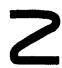
\includegraphics[keepaspectratio]{images/part002_ab1a0807.jpg}}

Since every band in a fully lattice-ordered space is itself a fully lattice-ordered space (Ch. II, §1, No.~5), one sees that the space \(L_{loc}^{1}\) is fully lattice-ordered; but it is worthwhile to recall that the supremum in \(L_{loc}^{1}\) of an uncountable family \((\dot{f}_{\alpha})\) of equivalence classes is not necessarily identical to the class of the upper envelope of the functions \(f_{\alpha}\) . However, we saw that for an increasing sequence \((f_{n})\) of locally \(\mu\) -integrable functions whose upper envelope f is locally \(\mu\) -integrable, \(f \cdot \mu\) is the supremum of the sequence of measures \((f_{n} \cdot \mu)\) in \(\mathcal{M}(T)\) (Cor. of Prop. 6).

Here is an interesting consequence of Corollary 3 of Th. 2:

PROPOSITION 9. --- Let \(\theta\) be a bounded complex measure; for \(\theta\) to be a positive measure, it is necessary and sufficient that \(\| \theta \| = \theta(1)\) .

The condition is obviously necessary. Conversely, suppose that \(\|\theta\|=\int d\theta\) , and denote by v a \(|\theta|\) -measurable function of absolute value 1 such that \(\theta=v\cdot|\theta|\) . Since \(\|\theta\|=\int d|\theta|\) (Ch. IV, §4, No.~7, Prop. 12) and \(\int d\theta=\int v\cdot d|\theta|\) (Th. 1), the hypothesis implies that \(\int(1-v)d|\theta|=0\) and therefore \(\int\mathcal{R}(1-v)d|\theta|=0\) . The function \(\mathcal{R}(1-v)\) , being positive, is therefore zero almost everywhere, which implies that v=1 almost everywhere and completes the proof.

